\definecolor{darkgreen}{rgb}{0.0, 0.5, 0.13}
\newcommand{\gct}{\color{darkgreen}\checkmark}
\newcommand{\rma}{\color{red}\ding{55}}
\newcommand{\bct}{\color{blue}\checkmark}
\title{NNPDF}
\author[Roy Stegeman]{}
\institute{University of Milan}
\date{PDF4LHC}

\subsection{Correlation and combination of PDF sets}

\begin{frame}{Self-correlation of PDF sets}
    	\begin{columns}[t]
        	\column{0.5\linewidth}
        	
		 Are PDF sets based on the same NNPDF methodology and underlying data fully correlated with respect to the data replicas?

        	\vspace{0.2cm}
			No, they are not fully correlated as a result of uncorrelated functional uncertainties.

		\vspace{0.2cm}
			\only<2>{If the correlation is higher, this means the functional uncertainty is smaller if compared to the data uncertainty.}

        	\column{0.5\linewidth}
        		\begin{center}
        		\begin{figure}
            		\captionsetup{format=smol}
            		\includegraphics<1>[width=\textwidth]{roy_pdf_correlations/nnpdf31_corr.pdf}
            		\includegraphics<2>[width=\textwidth]{roy_pdf_correlations/nnpdf31&40_corr.pdf}
            		\vspace{-0.9cm}
            		\caption{\tiny PDF-PDF self-correlation calculated with respect to data replicas, for sets based on the same NNPDF methodology and data, but different (random) initialization}        		
			\end{figure}
			\end{center}

    	\end{columns}
\end{frame}


\begin{frame}{Combination of PDF sets}
    	\begin{columns}[t]
        	\column{0.6\linewidth}

			At present PDF sets are combined under the assumption that they are fully correlated, can we instead combine the PDF sets in a correlated way?

        	\vspace{0.2cm}
			No, this can lead to arbitrarily small uncertainties if we combine repeated PDF determinations.

       	\column{0.4\linewidth}
       	\vspace{-2.7cm}
       	\begin{center}
       		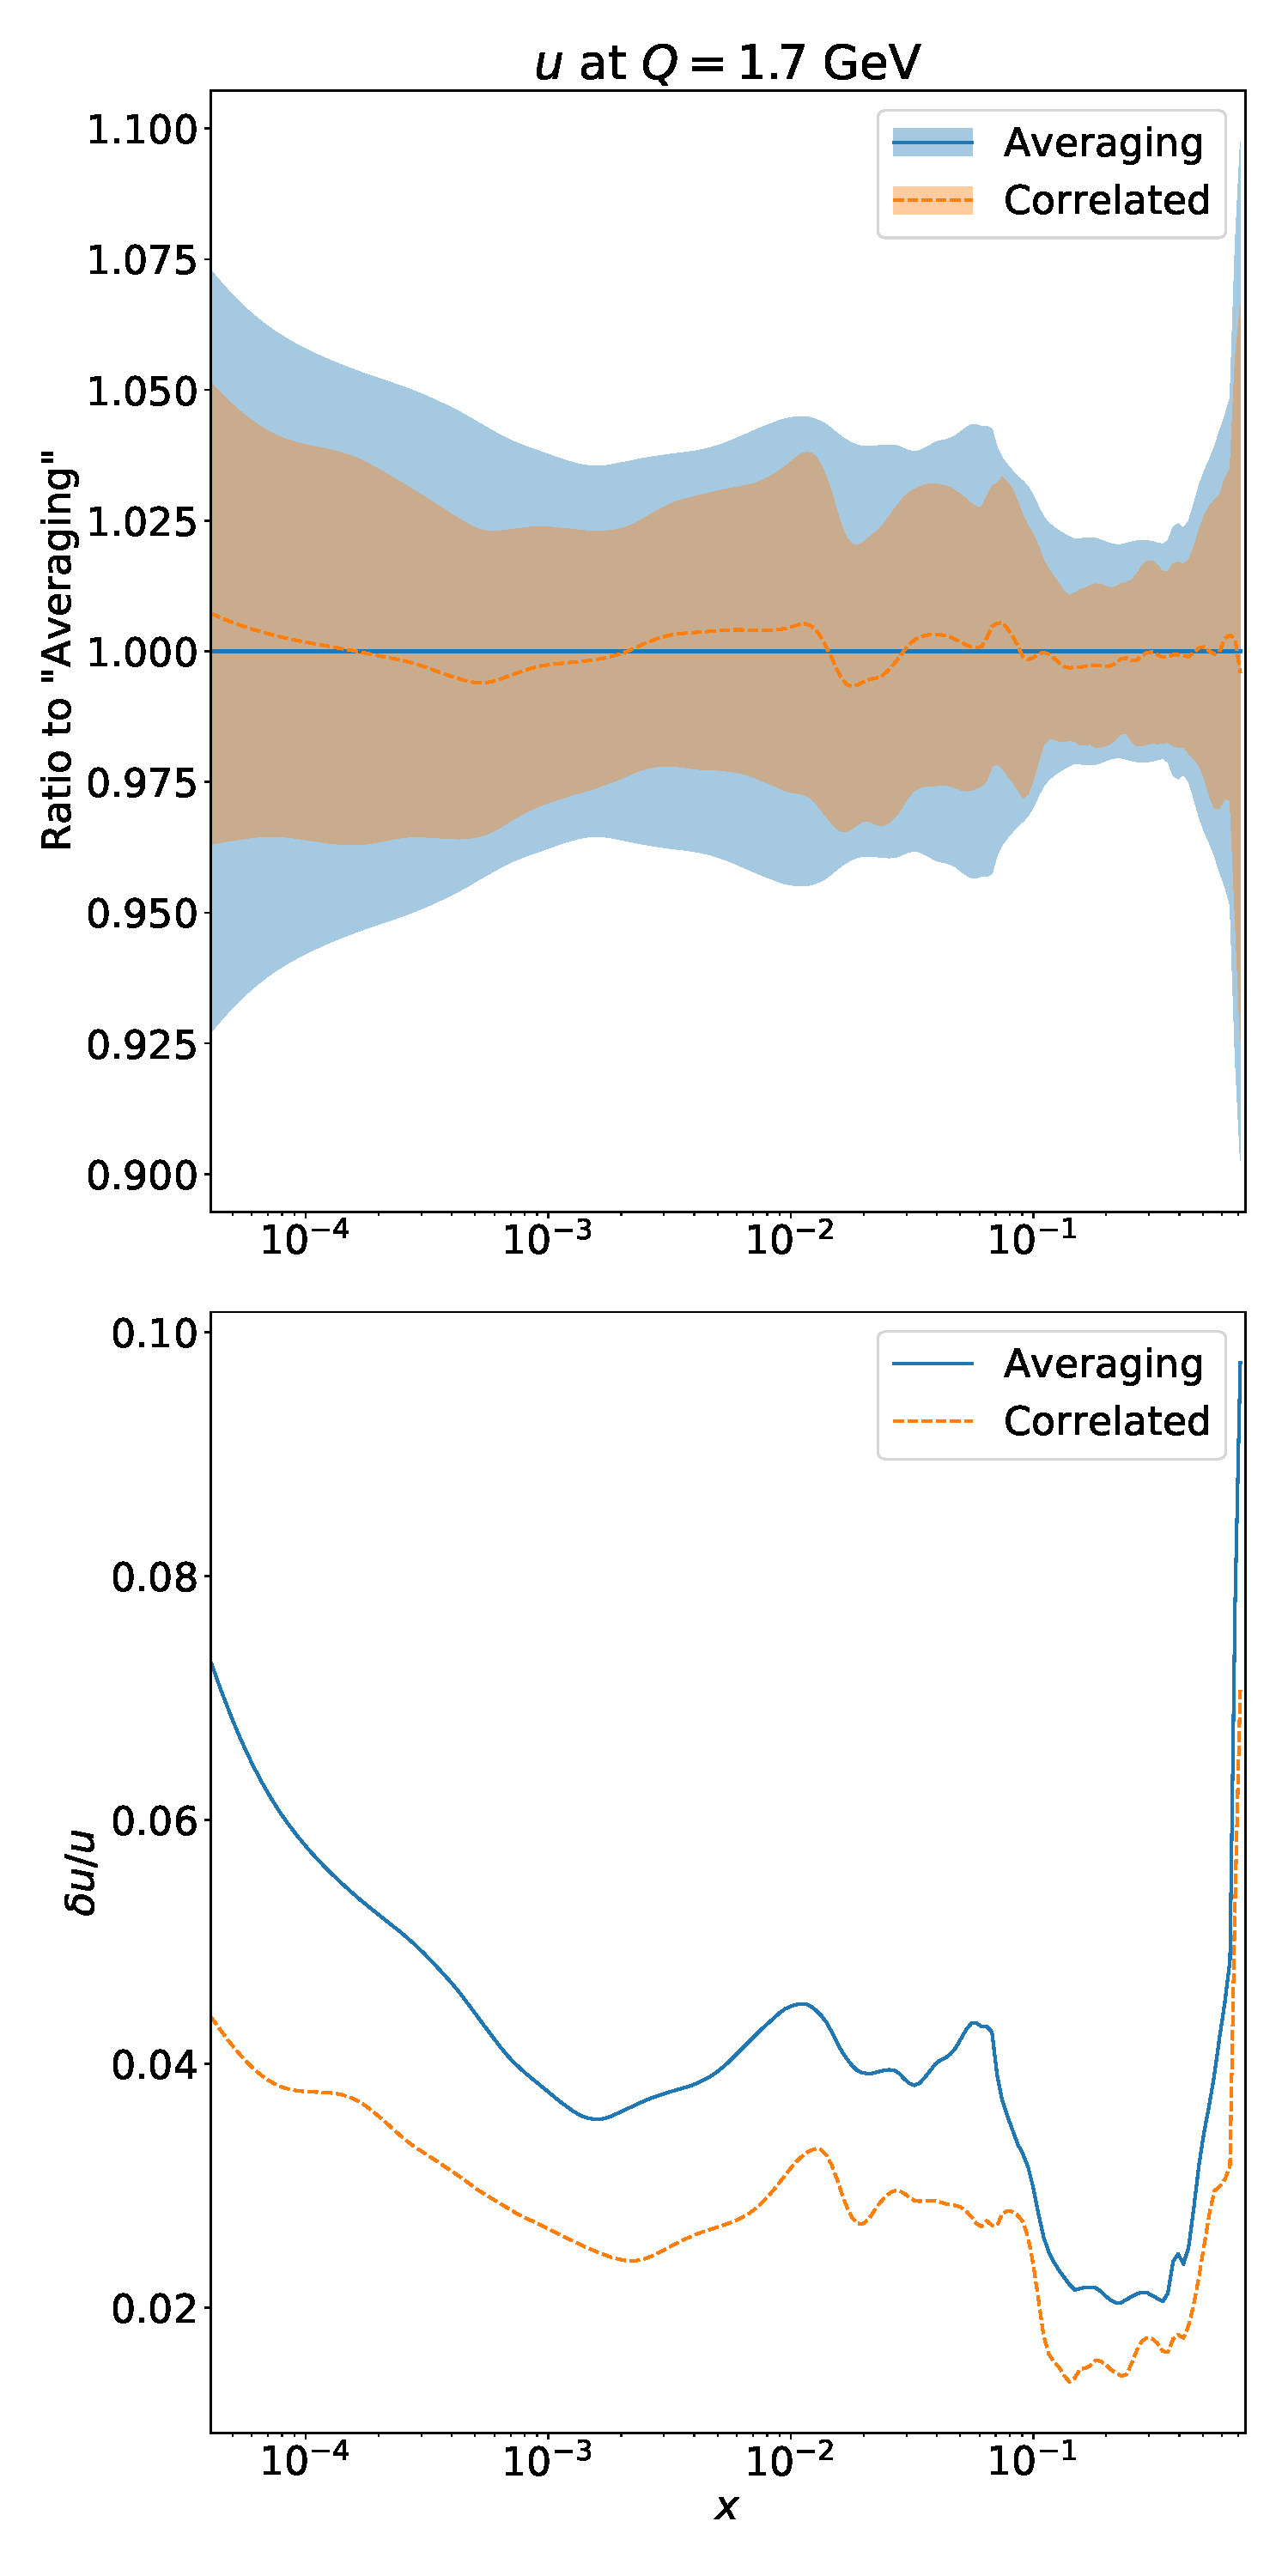
\includegraphics[height=1.15\textheight]{roy_pdf_correlations/ratio_2.pdf}
       	\end{center}
			
    	\end{columns}
\end{frame}

